
\chapter{Profiling Tool}
\label{chap:profiling-tool}


\section{Profiling a CUDA program running on a remote machine}

You can 
\begin{itemize}
  \item use nprof, running remotely, to profile a program on the remote machine, then copy the data back for loading 
  into the local Nvidia visual profiler
  
  \item using Nvidia visual profiler, or Nsight (Eclipse) to profile a remote machine. 
  
NOTE: Visual Profiler and nvprof will be deprecated in a future CUDA release
(still available in CUDA 10.0).
\item 
It is recommended to use next-generation tools NVIDIA Nsight Compute
(Sect.\ref{sec:nsight-compute}) for GPU profiling and NVIDIA Nsight Systems for
GPU and CPU sampling and tracing (Sect.\ref{sec:nsight}).

\end{itemize}

Here, we focus on using local Nsight to profile a remote program
\begin{enumerate}
  \item Run/ Profile Configurations: 
\end{enumerate}


\subsection{event}

An event is a countable activity, action, or occurrence on a device. It corresponds to a single hardware counter value which is collected during kernel execution. To see a list of all available events on a particular NVIDIA GPU, type nvprof --query-events.

\subsection{metric}

A metric is a characteristic of an application that is calculated from one or
more event values. To see a list of all available metrics on a particular NVIDIA
GPU, type nvprof --query-metrics. You can also refer to the metrics reference .


\subsection{limited profiling}

By default, the profiling tools collect profile data over the entire run of your application

To limit profiling to a region of your application, CUDA provides functions to
start and stop profile data collection. cudaProfilerStart() is used to start
profiling and cudaProfilerStop() is used to stop profiling IMPORTANT: To use
these functions you must include \verb!cuda_profiler_api.h! (or cudaProfiler.h
for the driver API).

Also, when using the start and stop functions, you also need to instruct the
profiling tool to disable profiling at the start of the application. For nvprof
you do this with the --profile-from-start off flag. For the Visual Profiler you
use the Start execution with profiling enabled checkbox in the Settings View.


\subsection{Nvidia NSight Compute CLI (x86\_64 only for version 1.0)}
\label{sec:nsight-compute}

Nvidia NSight Compute is the next-generation tools for GPU profiling; and NVIDIA
Nsight Systems for GPU and CPU sampling and tracing (Sect.\ref{sec:nsight}).


NVIDIA® Nsight Compute is an interactive kernel profiler for CUDA applications.
It provides detailed performance metrics and API debugging via a user interface
and command line tool (nv-nsight-cli).

The version 1.0 (using Nvidia driver toolkit 10.0) allows profiling
\verb!x86_64! [not Power9 machine yet] Window and Linux platforms locally (for data collection)
\begin{verbatim}
Linux x86_64
Windows x86_64
\end{verbatim}
or
from Windows, Linux, or MacOS hosts
\begin{verbatim}
Linux x86_64
Windows x86_64
MacOSX
\end{verbatim}
. It requires GPU
\begin{verbatim}
Pascal: GP10x (excluding GP100)
Volta: GV100
Turing: TU10x
\end{verbatim}

\url{https://docs.nvidia.com/nsight-compute/NsightComputeCli/index.html}


\section{gperf}
\label{sec:gperf}

The program must be compiled using \verb!-pg! option. 

For parallel applications only: if you want each parallel process to produce its
own output file, you will need to set the undocumented environment variable
\verb!GMON_OUT_PREFIX! to some non-null string

\begin{verbatim}

// ksh
setenv GMON_OUT_PREFIX 'gmon.out'

// bash
export GMON_OUT_PREFIX='gmon.out'
\end{verbatim}


Then, run the program normally, which will generate \verb!gmon.out! file at the end.

\begin{verbatim}
// for parallel program
% gprof myprog -s gmon.out.*
\end{verbatim}
\url{https://hpc.llnl.gov/software/development-environment-software/gprof}

\begin{verbatim}
gmon.out.18297 gmon.out.18300 gmon.out.9097
\end{verbatim}

Finally, we check the output file by passing the program name to \verb!gperf! and also the output file name

\begin{verbatim}
Serial
	 gprof myprog gmon.out
Parallel - one process only
	gprof myprog gmon.out.18302
Parallel - multiple processes
	gprof myprog gmon.out.18297 gmon.out.18300 gmon.out.9097
Parallel - all processes
	gprof myprog gmon.out.* 

\end{verbatim}


Gprof's output consists of a human-readable report produced from the binary
sampling file(s) created when the application was executed. By default the
report is written to stdout, which can always be redirected to a file with a
name of your choosing. For parallel programs, the report is a summation of the
files used to produce it.

\begin{enumerate}
  \item {\bf Flat Profile}:
  
  The functions are sorted first by decreasing run-time spent in them, then by
  decreasing number of calls, then alphabetically by name.
  
  \begin{verbatim}
Each sample counts as 0.01 seconds.  
  \end{verbatim}
  This sampling period estimates the margin of error in each of the time figures. 
  Here, each sample counts as 0.01 seconds suggesting  100 Hz sampling rate.
  
  So, a time figure that is not much larger than this is not reliable
  
  \item {\bf Graph Profile}:
  
  
  
\end{enumerate}




\section{PGI profile (PGI Accelerator)}
\label{sec:pgi-profile}

PGI Fortran provides a simple profiling feature for the compiler
targeting to Accelerator Programming Model (APM) when you compile the
code with \verb!-ta=nvidia,time! flag.  The profile library is linked
into the program so that the performance is collected when the program
is run. The collected information involves the elapsed time for the
accelerator regions and kernels; the time spent initializing the
device.

{\bf Example}:
\begin{verbatim}
Accelerator Kernel Timing data
c5.c
  test
    32: region entered 1 time
        time(us): total=1411909 init=1408006 region=3903
                  kernels=44 data=3859
        w/o init: total=3903 max=3903 min=3903 avg=3903
        35: kernel launched 1 times
            grid: [7x7]  block: [16x16]
            time(us): total=28 max=28 min=28 avg=28
        39: kernel launched 1 times
            grid: [7x7]  block: [16x16]
            time(us): total=16 max=16 min=16 avg=16
\end{verbatim}
The first information given from the above text is that the program
has one accelerator region, invoked once, at line 32 in routine
{\it test} of the file {\it c5.c}. The accelerator region spent
1411909us = 1.411 (sec). Of that, 1.40 (sec) is for the initializing
the device (including data movement), and 3.9(msec) executing the
kernels in the region. It means that most of the time spent moving
data.  The second information is that the accelerator region has 2
kernels, at line 35 and 39, each executed once (of course).

\begin{framed}
  The initialization cost is composed of the time spent in the
  NVIDIA runtime library and device drivers to initialize memory
  structures, and connect to the device. Normally, this cost only needs
  to be paid once per program execution. It ranges from 40 msec to 8 sec
  on one cluster initialization. To reduce this cost, you can run the
  program {\bf pgicudainit} in the background; it will keep open CUDA
  connection to the device driver, significantly reducing time for
  subsequent
  programs\footnote{\url{http://www.pgroup.com/lit/articles/insider/v1n2a1.htm}}. 
\end{framed}
\section{CUDA {\bf cudaprof}}
\label{sec:cuda-cudaprof}


{\bf cudaprof} is used in CUDA 2.3 and earlier, which displays the
summary of related {\bf profile counters} (or profile signals) to
kernels.
\textcolor{red}{The major limitation is that these counters are
  reported based on a single SM - SM zero, not the whole chip}.
It means that the value doesn't reflect the true number of events in
the whole-chip but are interpolated from a single SM.  So, if the work
loads are evenly distributed among SMs, we can expect the reported
values to reflect the behavior of the whole GPU. So, with 30 SMs in
C1060,
\textcolor{red}{to avoid large imbalance, we should use at least 120
  thread blocks in a single kernel launch}.

CUDA 2.3 has totally 21 counters for analyzing kernel performance.
\begin{enumerate}
\item \verb!gld 32b! 32-byte global memory load transactions
\item  \verb!gld 64b! 64-byte global memory load transactions
\item  \verb!gld 128b! 128-byte global memory load transactions
\item  \verb!gst 32b! 32-byte global memory store transactions
\item  \verb!gst 64b! 64-byte global memory store transactions
\item  \verb!gst 128b! 128-byte global memory store transactions
\item  \verb!local_load! = Local memory loads
\item  \verb!local store! =  Local memory stores
\item  \verb!branch! =  Number of branches
\item  \verb!divergent branch! =  Number of divergent branches
\item  \verb!instructions! Instructions executed
\item \verb!warp serialize! = Number of thread warps that has bank
  conflicts
\item  \verb!tlb miss! =  Number of TLB misses
\item ...
\end{enumerate}
At a single run, there are maximum 4 counters can be reported.  So, to
get all counters' values, {\bf cudaprof} need to run 5 times.
\textcolor{red}{ There are other important events that are not
  monitored by CUDA Profiler, e.g. data read from DRAM through device
  texture hardware.}

\begin{framed}
  The profiler {\bf cudaprof} is not a part of the CUDA SDK. To know
  which dynamic libraries that it uses, we can use {\it ldd} command
\begin{lstlisting}
  ldd /opt/local/cuda/cudaprof/bin/cudaprof
\end{lstlisting}

\end{framed}

We can define virtual counters named \verb!gld! and \verb!gst!
\verb!gld!~\citep{nagasaka2010}
\begin{verbatim}
gld = gld_32b + 2 x gld_64b + 4 x gld_128b

gst = gst_32b + 2 x gst_64b + 4 x gst_128b
\end{verbatim}
Under the assumption of ``coalesced'' memory address patterns, 
\begin{itemize}
\item one 32-bit access instruction needs one 128-byte transaction per
  warp
\item one 64-bit access instruction needs 2 128-byte transaction per
  warp
\item one 128-bit access instruction needs 4 128-byte transaction per
  warp.
\end{itemize}

The coefficients of the latter two counters reflect the ratio of the
chunk size to that of gld 32b (and gst 32b). Instead of the original
counters, we use gld and gst so that the number of independent
variables is reduced to nine, which would require less training data
for robust regression analysis

The number of all memory accesses \verb!mem! is defined as
\begin{verbatim}
mem = gld + gst + local_load + local_store.
\end{verbatim}

\begin{itemize}
\item Summary Table: how many times a kernel and runtime routines was
  called; and the time was spent aggregate in that routine. Additional
  information for kernels: branches, divergent branches, instruction
  throughput...

\item Width Plot: the horizontal is the GPU in which it show the
  amount of time spent on kernel call, data movement by GPU

\item Height Plot: the vertical is the GPU time spent on each kernel
  call or data movement; the method invocations are shown horizontally
  and time in that invocation vertically.

\item Summary Plot: show the fraction of time GPU spent in each
  routine or kernel, and data movement. 
\end{itemize}


\section{CUDA {\bf computeprof}}
\label{sec:cuda-computeprof}


Since CUDA 3.1, the profiler is renamed from {\bf cudaprof} to
{\bf computeprof}. This section describes how to use
\verb!computeprof! to optimize the kernels. Suppose that you have a
kernel, before you optimize it, you need to know the bottleneck in the
kernel.

\textcolor{red}{We will focus on Fermi C2050 only and lists out the
  optimal values}
\begin{enumerate}
\item memory throughput
  \begin{enumerate}
  \item device memory: 144 GB/sec
  \item constant memory: 
  \end{enumerate}
\item instruction throughput
  \begin{enumerate}
  \item \textcolor{blue}{ 1030 GFLOPS (fp32), 515 GFLOPS (fp64)}
  \item instructions:bytes
  \end{enumerate}
\item latency
\item combination of above
\end{enumerate}

\begin{figure}[hbt]
  \centerline{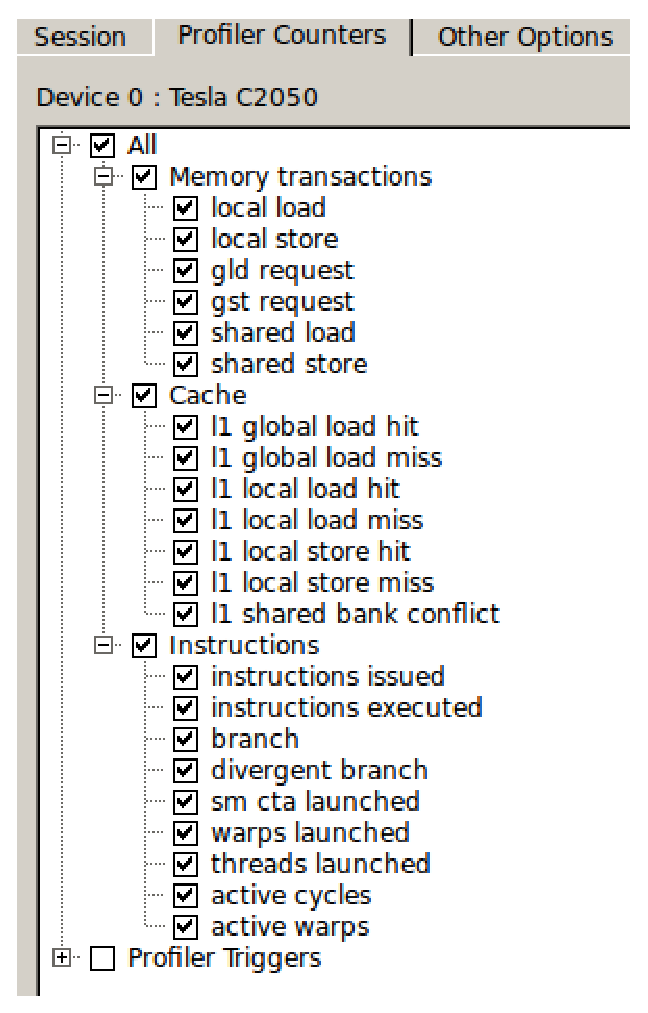
\includegraphics[height=9cm,
    angle=0]{./images/counter_profiler.eps}}
\caption{Counters in {\bf computeprof}}
\label{fig:counter_profiler}
\end{figure}

Like the old versions, most of the counters reported by the
\verb!computeprof!  are derived from the calculation of a single SM -
SM zero, not entire GPU, except L2 and DRAM counters. So, it's not
completely reflect the exact execution time. In a single run, it can
only collect a few counters and this number depends on the specific
counters selected. Normally, in CUDA 3.x,
\textcolor{red}{the Visual Profiler uses 9 runs} (when you request all
counters). If you use the command-line, the Compute Profiler, you need
to tell how many runs explicitly.

\begin{framed}
  \textcolor{red}{It is recommended to launch at least 2 times as many
    blocks as there are multiprocessors in the device which you're
    profiling}. E.g.: on Fermi, we need at least 28 thread blocks. 
  Two values for the same counter at different runs are not exactly
  the same. So, it's implicitly to understand that ``two counters
  being equal'' means ``with a small delta''. 

  By default, kernel launches are non-blocking. However, in the
  profiler, it's blocking so that the counters can be computed. With
  blocking kernels, the \verb!CPU time! is the sum of the
  \verb!GPU time! and the kernel launch overhead.
\end{framed}

\subsection{The GUI}
\label{sec:gui}

\begin{figure}[hbt]
  \centerline{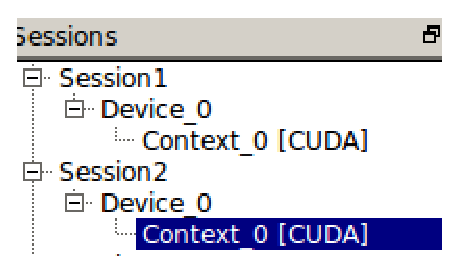
\includegraphics[height=2cm,
    angle=0]{./images/profiler_gui_1.eps}}
\caption{The Session, Device ID, and Context ID}
\label{fig:gui_1}
\end{figure}

At first you need to create a project, i.e. a single file. Then, each
time you run a benchmark, it is saved as a Session. During that
benchmark, one or more than device can be used. So the information for
a single device is saved into \verb!Device_0!, \verb!Device_1!... For
each device, the code can be CUDA (\verb!Context_0!) or OpenCL
(\verb!Context_1!), Fig.~\ref{fig:gui_1}.

After running the benchmark, if we right-click on the device being
used, e.g. \verb!Device_0!, and select ``Device level summary plot'',
we can see the cumulative GPU time for a method across all contexts
for a device, Fig.~\ref{fig:device_summary}. 

\begin{figure}[hbt]
  \centerline{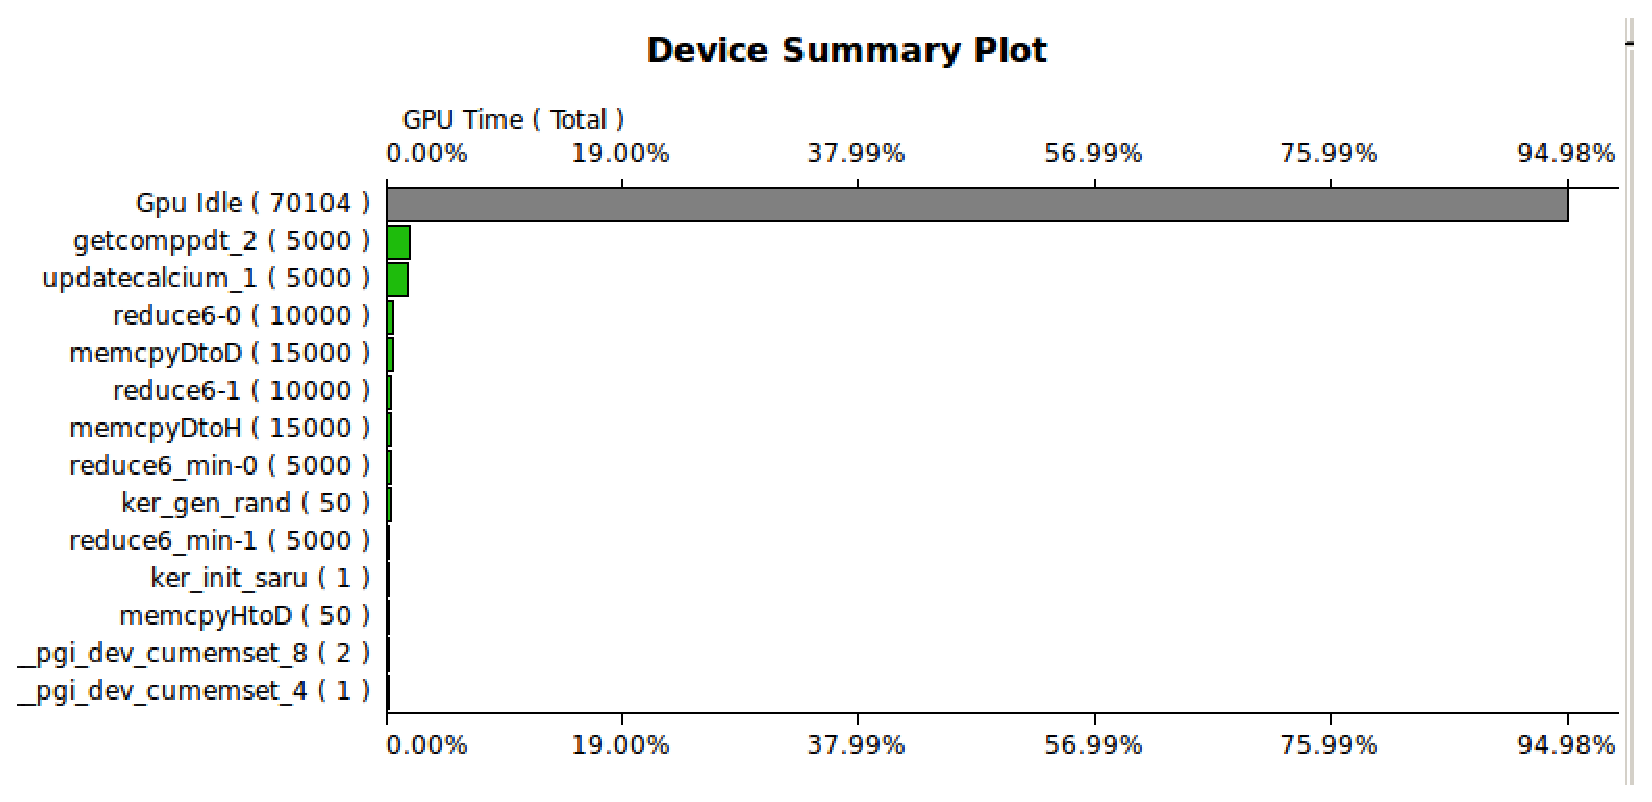
\includegraphics[height=5cm,
    angle=0]{./images/device_summary.eps}}
\caption{Device summary plot}
\label{fig:device_summary}
\end{figure}
  
In the Profiler output (information for a single kernel call in a
single SM)
\begin{enumerate}
\item {\bf GPU time}: the execution time for the Method
  
\item {\bf CPU time} : the sum of GPU time and CPU overhead to launch
  the kernel. All kernels launches are non-blocking by default. So, by
  default, it is the CPU overhead only. For blocking kernel calls,
  i.e. the CPU have to wait until the kernel finishes, CPU times is
  the sum of the GPU time and the CPU overhead. The CPU overhead in
  each kernel launch involves the time calling to CUDA Driver API and
  passing data argument to the device, before the kernel can be
  executed

  To understand the overhead involved in each kernel launch, we need
  to enable {\bf CUDA API trace} (which is not available in MacOS X),
  Fig.~\ref{fig:CUDA_API_trace}. Right-click on Context and then
  choose CUDA API trace. In this plot, the widths of the top bars show
  the GPU time for each kernel (methods) and the widths of the lower
  bars show the GPU time for CUDA driver API functions associated with
  that kernel call. \textcolor{red}{Pointer the cursors on the bar
    will show the attributes to the CUDA Driver API}, e.g. API name,
  time duration...

  \begin{figure}[hbt]
    \centerline{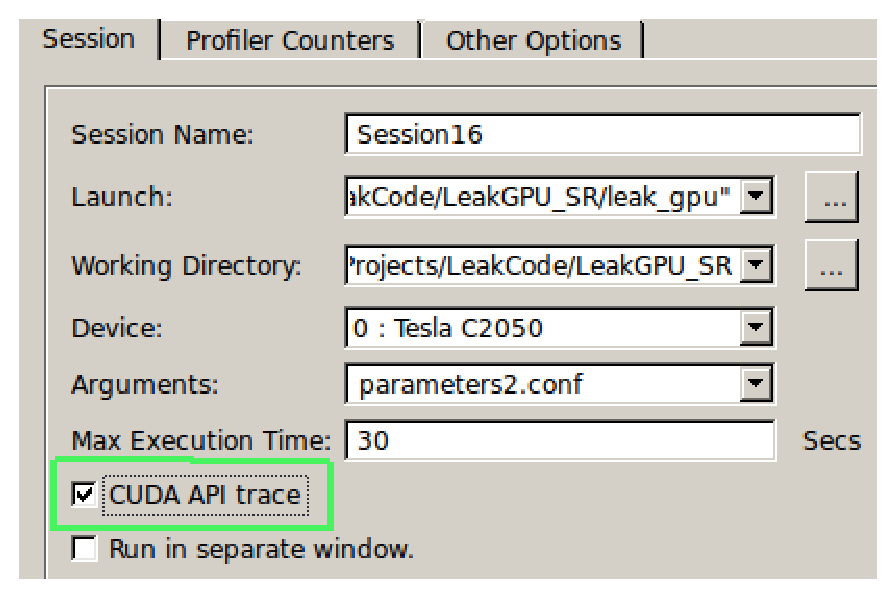
\includegraphics[height=3cm,
      angle=0]{./images/CUDA_API_trace.eps}}
    \caption{CUDA API trace}
    \label{fig:CUDA_API_trace}
  \end{figure}
  
\item {\bf Warp serialize}: the number of thread warps that serialize
  due to {\it memory/bank conflict} to either shared or constant
  memory. 
\item {\bf sm cta launched}: the number of threads blocks launched on
  a SM. 

\item \verb!L1 global load hit! and \verb!L1 global load miss!
  (Fermi) and global store transaction (C1060) = increment by 1 (per
  L1 cache line which is 128Byte)

  Global store transaction involves \verb!gst_32b!, \verb!gst_64b!,
  \verb!gst_128b! which are available in C1060 only. In Fermi, any
  type of access (coalesced/uncoalesced) will generate a large block
  transfer from main memory into L1 global memory cache. Each block of
  size 128Byte. 

\item \verb!gld request! and \verb!gst request! = counts the number
  of executed global memory read/store request which increment by 1
  (per warp)
  
\begin{verbatim}
gld_request = (l1_global_load_miss + l1_global_load_hit)
\end{verbatim}
  This value can be lower than the number of actual memory
  transactions.
  
\item \verb!instructions_issued! (include replays) and
  \verb!instructions_executed! (don't include replays) which
  increments 1 per warp

\item uncached global load transaction = increment by 1 per group of
  1, 2, 3, or 4 transactions
  
  It's better to use \verb!L2_read_request! counter (which increment
  by 1 per 32bytes memory load per GPU)

\item \verb!lmem! is like \verb!gmem!, except that writes are cached
  in L1. 
\end{enumerate}

\subsection{Environment variables}
\label{sec:envir-vari}

There are some environment variables:
\begin{enumerate}
\item \verb!COMPUTE_PROFILE!: set to either 0 or 1 to disable/enable
  profiling. 
\item \verb!COMPUTE_PROFILE_LOG! (or \verb!COMPUTE_PROFILE_LOG%d!) :
  the path to the profiling output (use \%d if (1) you use more than
  one device, and (2) you want separate profiler output for each
  device)
\item \verb!COMPUTE_PROFILE_CSV!: set to either 0 or 1 to
  disable/enable comma-separated version of the log output

\item \verb!COMPUTE_PROFILE_CONFIG!: the config file that tell which
  counters to measure. 
\end{enumerate}
\subsection{CPU overhead}
\label{sec:cpu-overhead}

At first, the function \verb!cuModuleLoadFatBinary! is called to load
cubin files in the current context. This function is called once for a
single context and take quite long (e.g. 440 ms),
Fig.~\ref{fig:CUDA_driver_API_1}.
\begin{figure}[hbt]
  \centerline{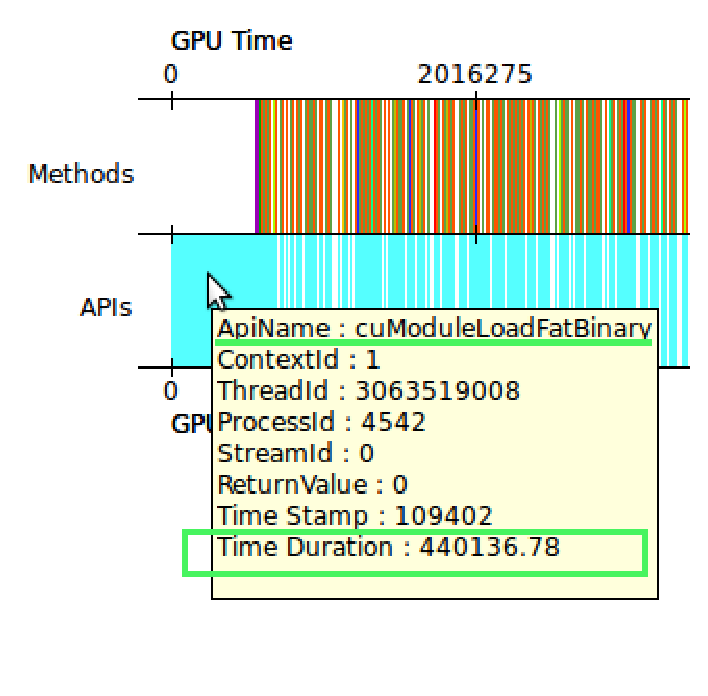
\includegraphics[height=5cm,
    angle=0]{./images/CUDA_driver_API_1.eps}}
\caption{The large overhead for the first API kernel call}
\label{fig:CUDA_driver_API_1}
\end{figure}

\begin{figure}[hbt]
  \centerline{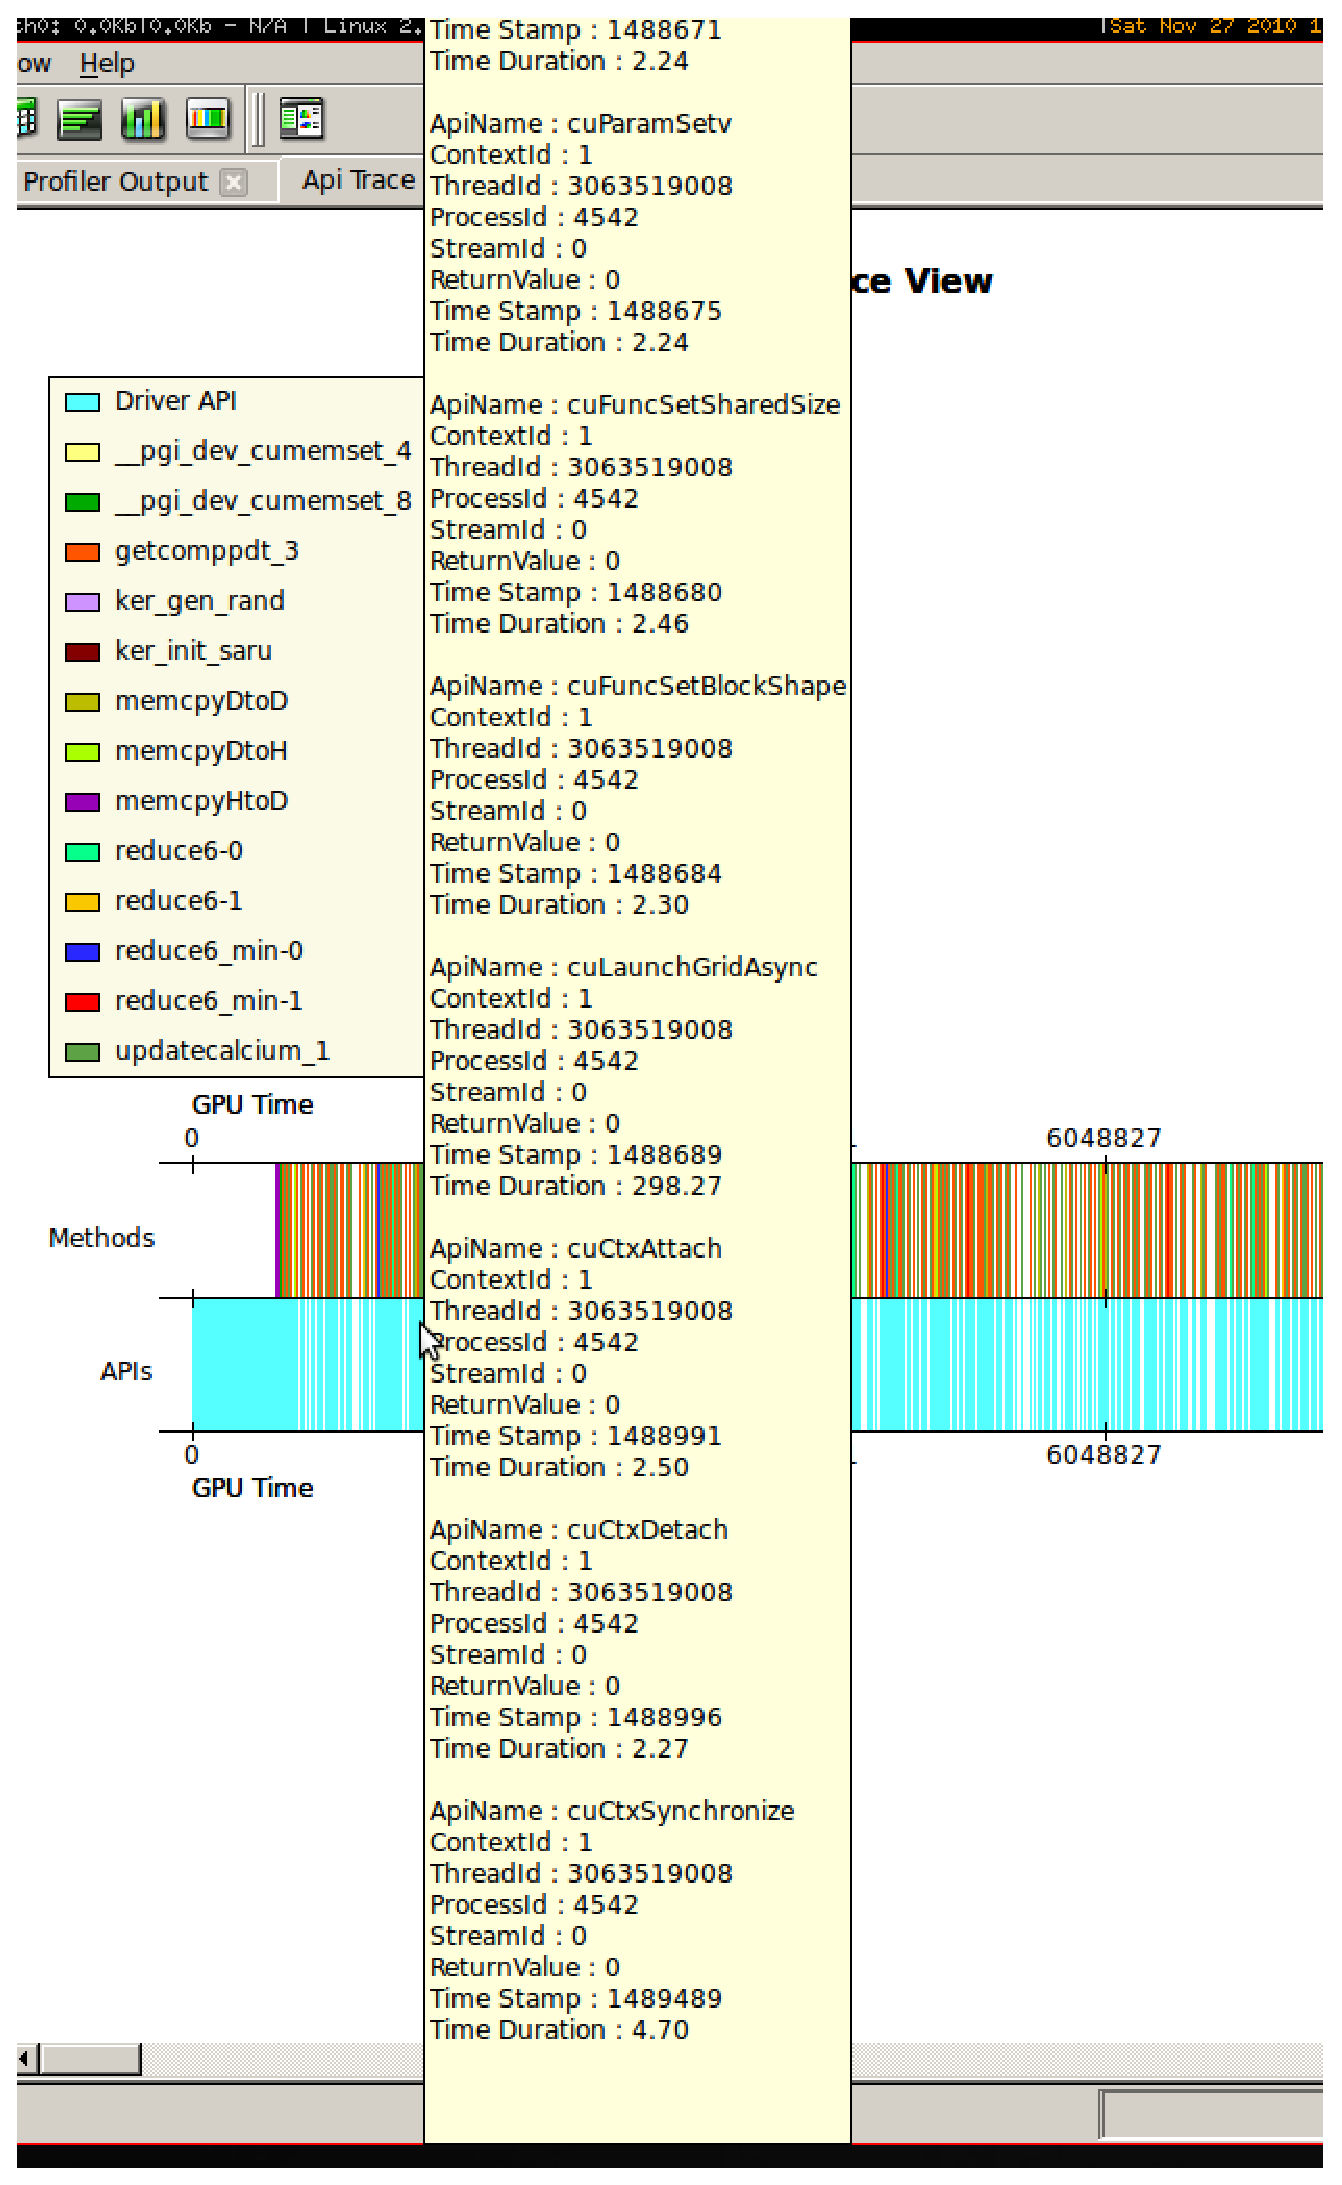
\includegraphics[height=5cm,
    angle=0]{./images/CUDA_driver_API_2.eps}}
  \caption{Then, next kernel call involves a number of CUDA Driver
    APIs call}
  \label{fig:CUDA_driver_API_2}
\end{figure}

For each kernel call, there is a number of CUDA Driver APIs need to be
invoked, Fig.~\ref{fig:CUDA_driver_API_2}.
\begin{enumerate}
\item 2-3 usec: \verb!cuParamSetSize!, \verb!cuParamSetV!,
  \verb!cuCtxAttach!, \verb!cuCtxDetach!, \verb!cuFuncSetSharedSize!,
  \verb!cuFuncSetBlockShape!, \verb!cuCtxSynchronize!. 

\item 250-300 usec: \verb!cuLaunchGridAsync! or \verb!cuLaunchGrid!
  which is invoked for every kernel call (one for asynchronous, one
  for synchronous).
\end{enumerate}

\begin{enumerate}
\item {\bf timestamp} = the time (usec) when kernel launches/memory
  transfers
\item {\bf gputstarttimestamp} = the time (usec) when the kernel
  starts execution
\item {\bf gputendtimestamp} = the time (usec) when the kernel ends
  execution
\item 
\end{enumerate}

\subsection{Summary Table - derived statistics}
\label{sec:summ-table-deriv}

There are some important statistics that we see in the Summary
Table. 
\begin{enumerate}
\item \verb!Method! = kernel function name or memcpyHtoD or memcpyDtoH or
  memcpyDtoD
\item \verb!# calls! = number of calls to Method during the
  simulation
\item \verb!GPU usec! = total GPU time in microseconds
\item \verb!%GPU time! = percent time that the whole simulation
  spending on GPU
  % \item {\bf CPU usec}: total CPU time in microseconds
\end{enumerate}

The derived statistics are the average taken over all the invocations
of that kernel (need to enable the average in Options/Session View
Settings/Summary Table tab - tick ``Show Average Data''). 
\begin{enumerate}
\item glob mem read throughput: global memory read throughput
\item glob mem write throughput: global memory write throughput
\item glob mem overall throughput
\item \verb!retire ipc! = (instructions executed) / (active cycle)
\item \verb!active warps/active cycle! = average number of warps that
  are active on a SM per cycle. 
\item \verb!L1 gld hit rate %! = percent of global load hit rate to
  L1 cache 
\begin{verbatim}
100 * (L1 global load hit count) / [ 
  (L1 global load hit count) + (L1 global load miss count) ]
\end{verbatim}
If caching-loads is used, count L1 misses. Otherwise, we count L2 read
request (NOTE L2 counters are for the entire chip, L1 counters are per
SM). 

\item \verb!texture hit rate %!
\begin{verbatim}
100 * (TEX_cache_requests - TEX_cache_misses) / (TEX_cache_request)
\end{verbatim}
\begin{verbatim}

\end{verbatim}
\end{enumerate}

\subsection{memory throughput}
\label{sec:memory-throughput}

For C1060:
\begin{itemize}
\item \verb!gld mem! = glob mem read throughput (GB/s)
\begin{verbatim}
gld_mem =  (total bytes read)/(GPU_time) 
\end{verbatim}
  where total bytes read is calculated using the profiler counters
  \verb!gld_32b!, \verb!gld_64b! and \verb!gld_128b!. 
\begin{verbatim}
total bytes read = gld_32 * 32 + gld_64 * 64 + gld_128 * 128
\end{verbatim}
  These quantities are not available in Fermi, since the read/write
  goes via L1/L2 caches. Instead, it reports cache hit/miss
  \verb!L1 global load hit/miss! and \verb!L1 local load hit/miss!.
\begin{verbatim}
total bytes read = DRAM reads * 32
\end{verbatim}

\item \verb!gstr mem! = glob mem write throughput (GB/s)
\begin{verbatim}
gstr_mem =  (total bytes write)/(GPU_time) 
\end{verbatim}
with (in Fermi)
\begin{verbatim}
total bytes write = DRAM writes * 32
\end{verbatim}

\item global mem overall throughput (GB/s)
\begin{verbatim}
glob mem overall throughput = gld_mem + gst_mem
\end{verbatim}
\end{itemize}

Note that 1 gigabyte refers to $10^9$ bytes in this calculation. This
is supported only for GPUs with compute capability 1.2 or higher.

\subsection{instruction throughput {\it instructions:bytes}}
\label{sec:instructions:bytes}

The ratio instructions:bytes tell how many issued instructions per a
single byte loaded. On Fermi, the perfect value (based on fp32
instructions) is
\begin{itemize}
\item \verb!~4.5:1! with ECC on
\item \verb!~3.6:1! with ECC off
\end{itemize}
\textcolor{red}{ perfect {\it instructions:bytes} ratio (based on fp64
  instructions only) ???? }

To compute number of issued instructions, take the number of
instructions issued times the number of threads in a warp
\begin{verbatim}
instructions_issued * 32
\end{verbatim}

To compute the number of bytes loaded, sum the number of L1 global
load hit and L1 global load miss, times the number of bytes that a
single transaction does
\begin{verbatim}
(L1 global load hit + L1 global load miss) * 128
\end{verbatim}

Read Sect.~\ref{sec:analys-modify-source} for example. 


References:
\begin{itemize}
\item \url{http://developer.download.nvidia.com/compute/cuda/3_0/toolkit/docs/visual_profiler_cuda/cudaprof.html}
\end{itemize}

\section{Analysis by modifying the source code}
\label{sec:analys-modify-source}

We can combine using Visual Profiler with modifying source code.  At
first, in the kernel, we need to tell which statement do memory
access, which statement do mathematical operations. Then, if they
don't have data-dependent control-flow or addressing, we can easily
modify the code, i.e.  disable some of them to measure the
\begin{itemize}
\item time spent accessing memory  (memory-only): remove all
  arithmetic maths
\item time spent on store-only: remove all arithmetic maths + memory
  loads
\item time spent in math-only: remove global memory access (NEED
  TRICK: instead of remove/comment out the memory store statements, we
  put them in a condition that always evaluate to FALSE. The
  conditions should depends on the value about to stored to prevent
  other optimizations that may automatically the condition,
  i.e. condition outcome should not be known to the compiler at
  compile time)
\begin{lstlisting}
if (value2stored < 0) {  // we know that
              // value2stored always positive
  ... do store operations here
}
\end{lstlisting}
or
\begin{lstlisting}
__global__ void fwd_3D( ..., intflag)
{
  ...
  value = temp + coeff* vsq;
  if( 1 == value * flag )
    g_output[out_idx] = value;
}
\end{lstlisting}
\end{itemize}
However, removing pieces of code is likely to affect registers count,
which in turns increase occupancy, and in the end, skew the
results. So, to make sure that we keep the occupancy, we need to check
the occupancy from the Visual Profiler before modifying the
codes. Then, after the modifications, we need to add shared memory to
match the unmodified kernels' occupancy.
\begin{lstlisting}
kernel<<<grid, blocks, smem, ...>>> (...)
\end{lstlisting}
Choose a suitable value of \verb!smem! to keep the occupancy
unchanged. 

Finally, it helps decide whether the kernel is memory of math
bound. Next, we sum up the total time when run the kernel for each
part separately, and the time when we enable all parts in the
kernel. By doing this, we can detect the overlapped the memory
operations with arithmetic. The common situations that may happen are
given in Fig.~\ref{fig:mem_math_bound}.

\begin{figure}[hbt]
  \centerline{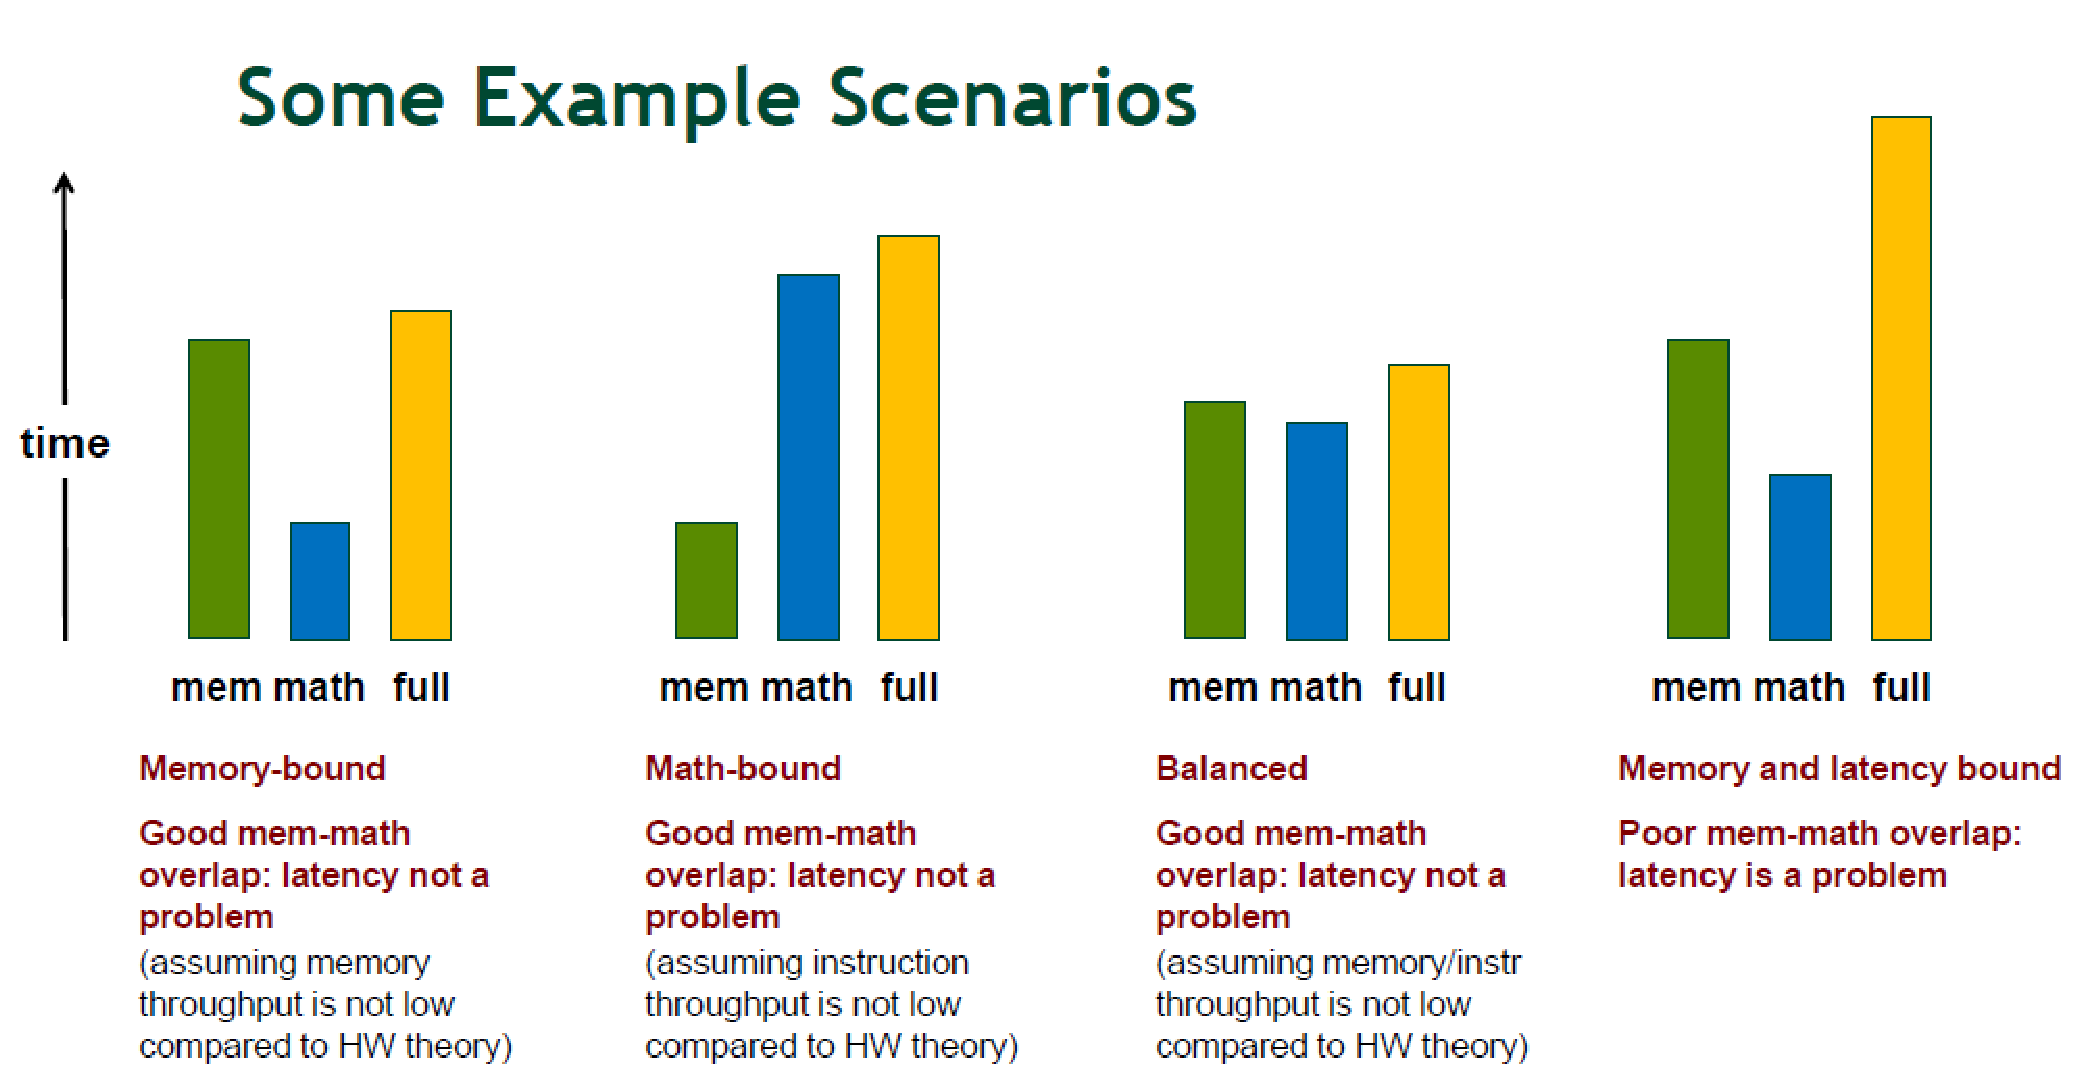
\includegraphics[height=5cm,
    angle=0]{./images/mem_math_bound.eps}}
\caption{Detect the overlap between mem and math operations}
\label{fig:mem_math_bound}
\end{figure}

{\bf Example}: The 3DFD kernel of the wave equation, use with fp32
operations 
\begin{enumerate}
\item Time (ms) 
  \begin{itemize}
  \item Full-kernel: 35.39 ms
  \item Mem-only: 33.27 ms
  \item Math-only: 16.25 ms
  \end{itemize}

\item Number of instructions issued:
  \begin{itemize}
  \item Full-kernel: 18,194,139
  \item Mem-only: 7,497,296
  \item Math-only: 16,839,792
  \end{itemize}

\item Memory access transactions:
  \begin{itemize}
  \item Full-kernel: 1,708,032
  \item Mem-only: 1,708,032
  \item Math-only: 0
  \end{itemize}
\end{enumerate}

So, we obtain
\begin{enumerate}
\item instr:byte ratio = \verb!~ 2.66!

\item good overlap between math and mem: $35.39-33.27 = 2.12$ msec of
  math-only time (i.e. 13\%) are not overlapped with mem. 

\item App memory throughput:
\begin{verbatim}
mem_transaction * 128 / kernel_time
\end{verbatim}
or 
\begin{verbatim}
1,708,032 * 128 / 35.39 = 6177680 bytes/sec
                        = 6.2 GB/sec
\end{verbatim}
while the theory peak is 114 GB/sec
\end{enumerate}

Conclusion: 
\begin{enumerate}
\item Code is memory-bound
\item Latency could be an issue, i.e. need more active threads 
\item Optimization should focus on memory throughput first, as math
  contributes very little to total time (2.12 out of 35.39 msec)
\end{enumerate}


\section{NVIDIA Visual Profiler: nvvp}
\label{sec:nvvp}

NVIDIA Visual profiler (nvvp) can be used asn either a stand-alone tool, or is
integrated into NVIDIA NsightTM Eclipse Edition (nsight).

The Visual Profiler displays a timeline of your application's activity on both
the CPU and GPU so that you can identify opportunities for performance
improvement.

The Visual Profiler will analyze your application to detect potential performance bottleneck

\begin{verbatim}
nvvp -vm /usr/lib64/jvm/jre-1.8.0/bin/java


// install openjdk-8-jre 
apt-get install openjdk-8-jre

nvvp -vm /usr/lib/jvm/java-8-openjdk-amd64/jre/bin/java
\end{verbatim}

\section{NSight Eclipse edition}
\label{sec:nsight}

NVIDIA Nsight Systems is used for GPU and CPU sampling and tracing.

It also include Nvidia visual profiler (Sect.\ref{sec:nvvp}).
The Visual Profiler is located in the Profile Perspective and is activated when
an application is run in profile mode.


\subsection{Changes (release)}

From CUDA 10.0:
\begin{enumerate}
  \item support CC 7.5
  
  \item Profiler supports version 3 of NVIDIA Tools Extension API (NVTX). This
  is a header-only implementation of NVTX version 2.
  
  \item 
\end{enumerate}

 
\section{CUDA {\bf nvprof}}
\label{sec:nvprof}
\label{sec:profiler-nvprof}

Note that Visual Profiler and nvprof will be deprecated in a future CUDA
release. It is recommended to use next-generation tools NVIDIA Nsight Compute
for GPU profiling and NVIDIA Nsight Systems for GPU and CPU sampling and
tracing.

nvprof is a command-line profiler available for Linux, Windows, and OS X.
nvprof is added from CUDA 5.0.

\begin{verbatim}
nvprof -o profiler_mps_mgpu$lrank.pdm ./application_exe
\end{verbatim}


nvprof knows how to profile any CUDA-based program, e.g. written in C, Fortran,
or even OpenACC programs (which have no explicit kernels), or even programs that
generate PTX assembly kernels internally.
 
nvprof can be used to profile a program running on a remote computer.
Simply connect to the remote machine (using ssh, for example), and run your
application under nvprof.
\begin{verbatim}
--output-profile command-line option, 
	you can output a data file for later import into either 
		nvprof or 
		the NVIDIA Visual Profiler. 
	This means that you can capture a profile on a remote machine, 
	and then visualize and analyze the results on your desktop 
	in the Visual Profiler (see “Remote Profiling” for more details).

\end{verbatim}

\url{https://docs.nvidia.com/cuda/profiler-users-guide/index.html}

\url{https://devblogs.nvidia.com/cuda-pro-tip-nvprof-your-handy-universal-gpu-profiler/}

\subsection{Output to file}




Now, Make a script and run on a remote machine
\begin{verbatim}
nvprof --export-profile timeline.prof <app> <app args>

nvprof --metrics achieved_occupancy,ipc -o metrics.prof <app> <app args> 


nvprof --kernels <kernel specifier> --analysis-metrics -o analysis.prof <app> <app args> 

\end{verbatim}
Then copy the multiple files back to local machine, which then can be loaded
into Nvidia Visual Profiler (nvvp).

IMPORTANT:  CPU profiling is not supported in multi-process mode.
However, in multi-threading, we need to use CPU thread tracing
\verb!-cpu-thread-tracing! on during measurement (LIMITATION: not supported on
Windows). Recording this information is necessary if the application uses
multiple CPU threads and at least two of these threads call the CUDA API.
Currently, only POSIX threads (Pthreads) are supported.
Note: CPU thread tracing starts after the first CUDA API call, from the thread
issuing this call.
Therefore, the application must call e.g. cuInit from its main thread before
spawning any other user threads that call the CUDA API.




To collect performance data about your application, the Visual Profiler must be
able to execute your application repeatedly in a deterministic manner. Due to
software and hardware limitations, it is not possible to collect all the
necessary profile data in a single execution of your application.
Each time your application is run, it must operate on the same data and perform
the same kernel and memory copy invocations in the same order.


\begin{verbatim}
// just  collect a timeline
// we should NOT combine with other option, as they affect the real timeline

nvprof --export-profile timeline.prof <app> <app args>
\end{verbatim}

We can copy this file back to the host system and then import it into the Visual
Profiler

\begin{verbatim}
// collect  events or metrics for all kernels
// profiles all kernels launched on all visible CUDA devices by default

nvprof --metrics achieved_occupancy,ipc -o metrics.prof <app> <app args> 


// limit the profiling to
// 1. certain device 
// 2. certain kernels and/or at given invocation 
Example:
nvprof --devices 0 --metrics ipc
        --kernels "1:foo:bar:2" --events local_load a.out
        

--devices <device IDs> 
         applies to --events, --metrics, --query-events, and 
          --query-metrics that follows it

--kernels <kernel filter> 
         applies to --events and --metrics options that follows it.

	NOTE: <kernel filter> can be
	<kernel name>
	
	or
	
	<context id/name>:<stream id/name>:<kernel
        name>:<invocation>
        
    NOTE: Each string in the angle brackets can be 
    a standard Perl regular expression. 
    Empty string matches any number or character combination.

	NOTE: Invocation number n indicates the nth invocation of the kernel.
	
	Example:
	:::3 will match the 3rd invocation of every kernel.
	    
\end{verbatim}
 
IMPORTANT: Collecting events or metrics for all kernels will significantly
change the overall performance characteristics of the application because all
kernel executions will be serialized on the GPU.

\begin{verbatim}
// Unified Memory


// ... on multiple-GPU
// IF the two GPU  without P2P support between any pair of devices that support Unified Memory
// then indeed managed memory allocations are placed in zero-copy memory. 
//   and In this case Unified Memory profiling is not supported
// BUT when the environment variable CUDA_MANAGED_FORCE_DEVICE_ALLOC 
//     can be set to force managed allocations to be in device memory and 
//     to enable migration on these hardware configurations. In this case Unified Memory profiling is supported.


// If the two GPU with Peer2Peer support
//  Normally, using the environment variable CUDA_VISIBLE_DEVICES is 
//  recommended to restrict CUDA to only use those GPUs that have P2P support.



\end{verbatim}

\subsection{Output to standard output}

\begin{verbatim}
//simplest
nvprof ./myApp

 ==9261== Profiling application: ./tHogbomCleanHemi
 ==9261== Profiling result:
    Time(%)      Time     Calls       Avg       Min       Max  Name
     58.73%  737.97ms      1000  737.97us  424.77us  1.1405ms  subtractPSFLoop_kernel(float const *, int, float*, int, int, int, int, int, int, int, float, float)
     38.39%  482.31ms      1001  481.83us  475.74us  492.16us  findPeakLoop_kernel(MaxCandidate*, float const *, int)
      1.87%  23.450ms         2  11.725ms  11.721ms  11.728ms  [CUDA memcpy HtoD]
      1.01%  12.715ms      1002  12.689us  2.1760us  10.502ms  [CUDA memcpy DtoH]



// add which GPU each kernel ran, as well as the grid dimensions used for each launch.
nvprof --print-gpu-trace ./myApp

==4125== Profiling application: ./nbody --benchmark -numdevices=2 -i=1
==4125== Profiling result:
   Start  Duration            Grid Size      Block Size     Regs*    SSMem*    DSMem*      Size  Throughput           Device   Context    Stream  Name
260.78ms     864ns                    -               -         -         -         -        4B  4.6296MB/s   Tesla K20c (0)         2         2  [CUDA memcpy HtoD]
260.79ms     960ns                    -               -         -         -         -        4B  4.1667MB/s  GeForce GTX 680         1         2  [CUDA memcpy HtoD]
260.93ms     896ns                    -               -         -         -         -        4B  4.4643MB/s   Tesla K20c (0)         2         2  [CUDA memcpy HtoD]
260.94ms     672ns                    -               -         -         -         -        4B  5.9524MB/s  GeForce GTX 680         1         2  [CUDA memcpy HtoD]
268.03ms  1.3120us                    -               -         -         -         -        8B  6.0976MB/s   Tesla K20c (0)         2         2  [CUDA memcpy HtoD]
268.04ms     928ns                    -               -         -         -         -        8B  8.6207MB/s  GeForce GTX 680         1         2  [CUDA memcpy HtoD]
268.19ms     864ns                    -               -         -         -         -        8B  9.2593MB/s   Tesla K20c (0)         2         2  [CUDA memcpy HtoD]
268.19ms     800ns                    -               -         -         -         -        8B  10.000MB/s  GeForce GTX 680         1         2  [CUDA memcpy HtoD]
274.59ms  2.2887ms             (52 1 1)       (256 1 1)        36        0B  4.0960KB         -           -   Tesla K20c (0)         2         2  void integrateBodies(vec4::Type*, vec4::Type*, vec4::Type*, unsigned int, unsigned int, float, float, int) [242]
274.67ms  981.47us             (32 1 1)       (256 1 1)        36        0B  4.0960KB         -           -  GeForce GTX 680         1         2  void integrateBodies(vec4::Type*, vec4::Type*, vec4::Type*, unsigned int, unsigned int, float, float, int) [257]
276.94ms  2.3146ms             (52 1 1)       (256 1 1)        36        0B  4.0960KB         -           -   Tesla K20c (0)         2         2  void integrateBodies(vec4::Type*, vec4::Type*, vec4::Type*, unsigned int, unsigned int, float, float, int) [275]
276.99ms  979.36us             (32 1 1)       (256 1 1)        36        0B  4.0960KB         -           -  GeForce GTX 680         1         2  void integrateBodies(vec4::Type*, vec4::Type*, vec4::Type*, unsigned int, unsigned int, float, float, int) [290]

Regs: Number of registers used per CUDA thread.
SSMem: Static shared memory allocated per CUDA block.
DSMem: Dynamic shared memory allocated per CUDA block.
\end{verbatim}

%%% Local Variables: 
%%% mode: latex
%%% TeX-master: "gpucomputing"
%%% End: 

